\documentclass{article}

\usepackage[a4paper,left=18mm,right=18mm,top=20mm,bottom=18mm]{geometry}
\usepackage[italian]{babel}

\usepackage{titling}
\usepackage{graphicx}
\usepackage{subcaption}

\title{Report analisi dell'aria}
\author{David Guzman Piedrahita e Marco Vinciguerra}
\date{\today}

\makeatletter         
\def\@maketitle{
\noindent\begin{minipage}{\textwidth}
\begin{minipage}[c]{0.8\textwidth}
\begin{center}
{\Huge \bfseries \sffamily \@title }\\[4ex] 
{\Large  \@author}\\[4ex] 
\@date\\[0ex]
\end{center}
\end{minipage}\hfill
\begin{minipage}[c]{0.2\textwidth}
\raggedleft

\includegraphics[width = 20mm]{logo.png}\\[0.1ex]

\includegraphics[width = 25mm]{UniBg-logo.jpg}
\end{minipage}
\end{minipage}
}
\makeatother


\begin{document}

\maketitle

\par\noindent\rule{\textwidth}{0.4pt}
\textbf{Abstract:} Paper preliminare per la tesi di laurea
\par\noindent\rule{\textwidth}{0.4pt}

\section{Introduzione}
La fase iniziale del progetto consiste nell'analisi nell'arco temporale 2018-2020 dei dati 
forniti dal sito ARPAL relativi allo studio del $NH_{3}$ e dei particolati atmosferici $PM_{10}$ e $PM_{2.5}$ al 
fine di dimostrare i risultati positivi e la diminuzione dell'inquinamento dell'aria 
dovuti dal Covid19 in Lombardia. Le mappe della delle stazioni che rilevano gli inquinanti e meteo sono le 
seguenti:
\begin{figure}
    \centering
    \begin{subfigure}{.5\textwidth}
      \centering
      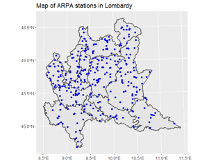
\includegraphics[width=.7\linewidth]{Lpollution.png}
      \caption{Stazioni degli inquinanti}
      \label{fig:sub1}
    \end{subfigure}%
    \begin{subfigure}{.5\textwidth}
      \centering
      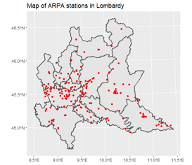
\includegraphics[width=.7\linewidth]{Lweather.png}
      \caption{Stazioni del meteo}
      \label{fig:sub2}
    \end{subfigure}
    \caption{A figure with two subfigures}
    \label{fig:test}
    \end{figure}

\section{Analisi preliminare dei dati per gli inquinanti}
La fase iniziale del progetto consiste nel cercare le centraline in Lombardia
che misurano contemporaneamente $NH_{3}$, $PM_{10}$ e $PM_{2.5}$ oppure solo due di essi
(sono ammessi dei dati mancanti sporadicamente per entrambi i casi).
Le centraline che misurano tutti e 3 sono solamente 6 e sono le seguenti:
\begin{itemize}
    \item Cremona via Fatebenefratelli (ID station: 677)
    \item Schivenoglia (ID station: 703)
    \item Sannazzaro de Burgondi Agip (ID station: 693)
    \item Pavia via Folperti (ID station: 642)
    \item Milano Pascal Citta Studi (ID station: 705)
    \item Moggio (ID station: 681)
\end{itemize}
mentre le stazioni che ne misurano solo due sono in totale 26.
Per ognuno di essi è stato calcolato quanti giorni tra il 2018 e il 2020 sono assenti
$NH_{3}$, $PM_{10}$ e $PM_{2.5}$ e quanti giorni sono assenti tutti e 3 contemporaneamente
(allegata con il nome MissingFromTheBeginning.csv).
In allegato c'è una tabella che descrive cosa viene misurato in ognuna
delle centraline prese in considerazione precedentemente (presencetableRed.csv).
Per ogni centralina che presenta tutti e 3 i regressori di interesse è stato fatto
un plot della serie storica e in presenza di un dato mancante in corrispondenza
di uno specifico giorno è stata tracciata una linea verticale blu.
Il risultato della mappa della Lombardia in funzione di tutte le centrali che misurano 2 o più inquinanti che 
vengono presi in considerazione è il seguente:

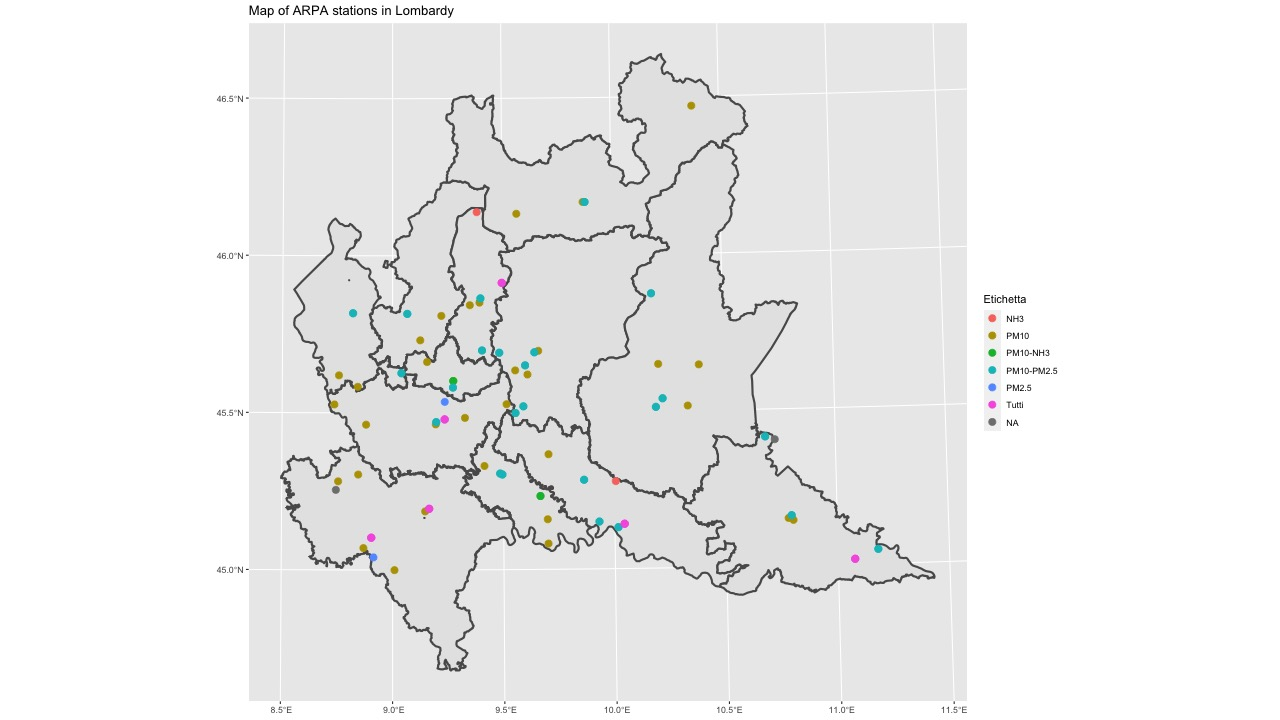
\includegraphics[scale=0.35]{mappina.jpeg}

Ecco un esempio di una  delle 6 migliori centraline con un numero accettabile di dati mancanti e una con
un numero molto alto di dati mancanti (sempre appartenente alla lista delle 6 migliori centrali):

\begin{figure}[]
    \centering
    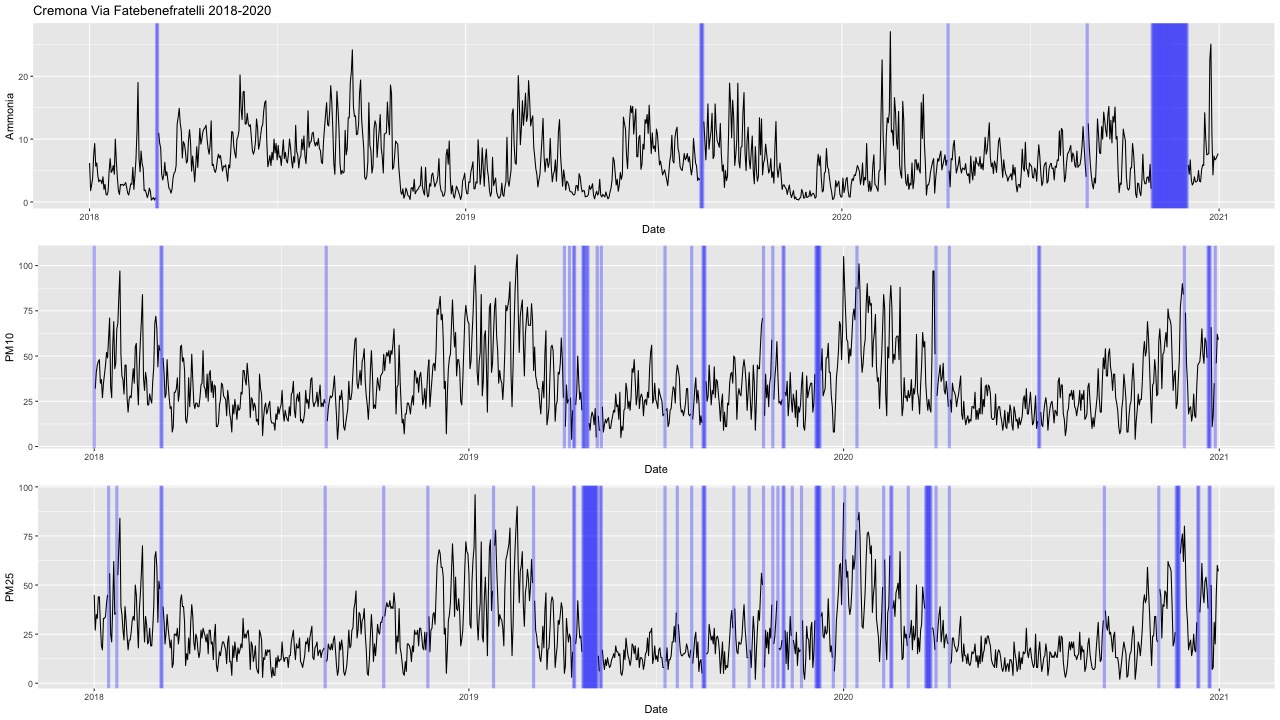
\includegraphics[scale=0.35]{Cremona Via Fatebenefratelli 2018-2020 .jpeg} 
    \caption{Cremona Via Fatebenefratelli 2018-2020, Mancanti Ammonia: 2, PM10: 4, PM25: 7, tutti e 3 contemporaneamente: 2}
    \centering
    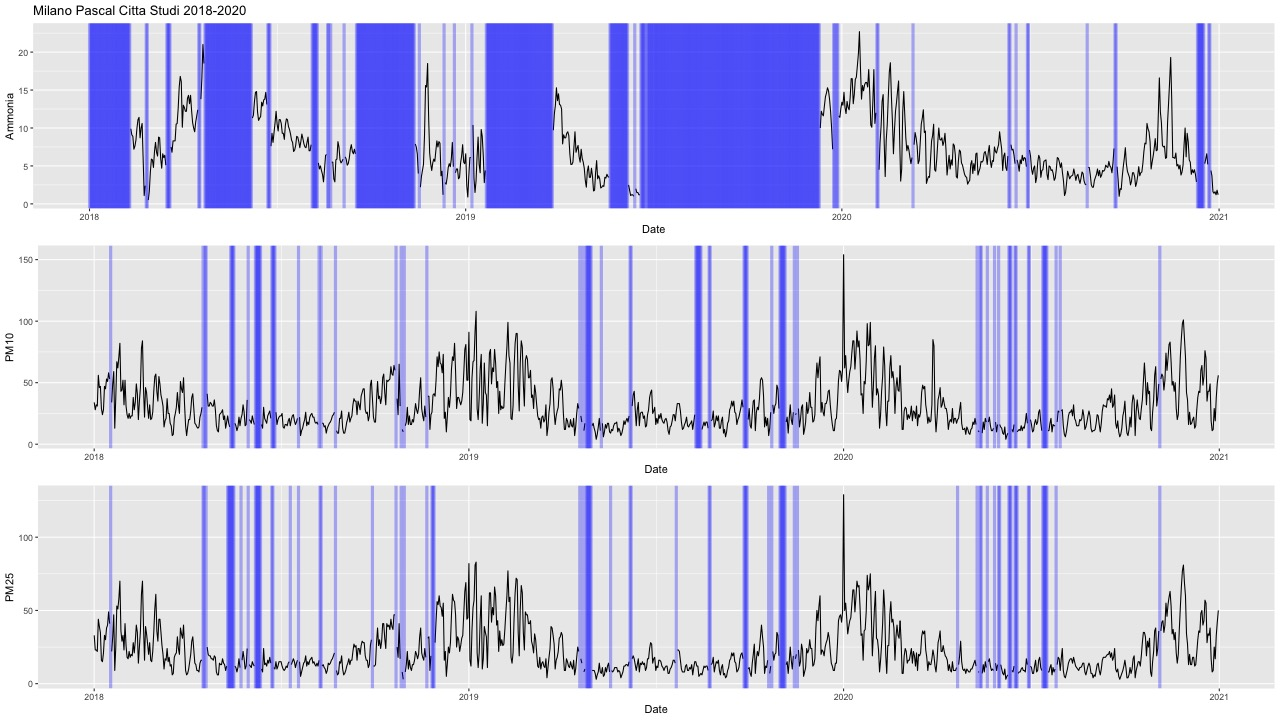
\includegraphics[scale=0.35]{Milano Pascal Citta Studi 2018-2020 .jpeg}
    \caption{Milano Pascal Citta Studi 2018-2020, Mancanti Ammonia: 167, PM10: 27, PM25: 34, tutti e 3 contemporaneamente: 14}
\end{figure}

\section{Analisi dei dati per il meteo}
Successivamente è stata cercata per ogni centralina che misura gli inquinanti, le due  
stazioni meteo più vicine che misurassero contemporaneamente velocità del vento (wind speed), direzione del vento (wind direction), 
temperatura (temperature) e precipitazioni (rainfall).
\end{document}
